%%% template.tex
%%%
%%% This LaTeX source document can be used as the basis for your technical
%%% paper or abstract. Intentionally stripped of annotation, the parameters
%%% and commands should be adjusted for your particular paper - title, 
%%% author, article DOI, etc.
%%% The accompanying ``template.annotated.tex'' provides copious annotation
%%% for the commands and parameters found in the source document. (The code
%%% is identical in ``template.tex'' and ``template.annotated.tex.'')

\documentclass[conference]{acmsiggraph}

\usepackage{authblk}
\usepackage[]{algorithm2e}

\TOGonlineid{45678}
\TOGvolume{0}
\TOGnumber{0}
\TOGarticleDOI{1111111.2222222}
\TOGprojectURL{}
\TOGvideoURL{}
\TOGdataURL{}
\TOGcodeURL{}


\usepackage{color}
\newcommand{\YOON}[1]{
	\textcolor{blue}{\bfseries{YOON's comment: {#1}}}
}


\title{Performance Driven Redundancy Optimization of Data Layouts for Walkthrough Applications}

%\author[1]{Zachary DeStefano\thanks{zdestefa@uci.edu}}
%\author[1]{Shan Jiang\thanks{sjiang1714@gmail.com}}
%\author[1]{Gopi Meenakshisundaram\thanks{gopi.meenakshisundaram@gmail.com}}
%\author[2]{Sung-Eui Yoon\thanks{toinsert}}
%\pdfauthor{Zachary DeStefano,Shan Jiang,Gopi Meenakshisundaram,Sung-Eui Yoon}
\pdfauthor{}
\author{}
%\affil[1]{University of California, Irvine}
%\affil[2]{KAIST}

\keywords{Data Layout Problem, Out-Of-Core Rendering, Cache Oblivious Mesh Layout, Redundant Data Layout, Walkthrough Application}

\begin{document}

%% \teaser{
%%   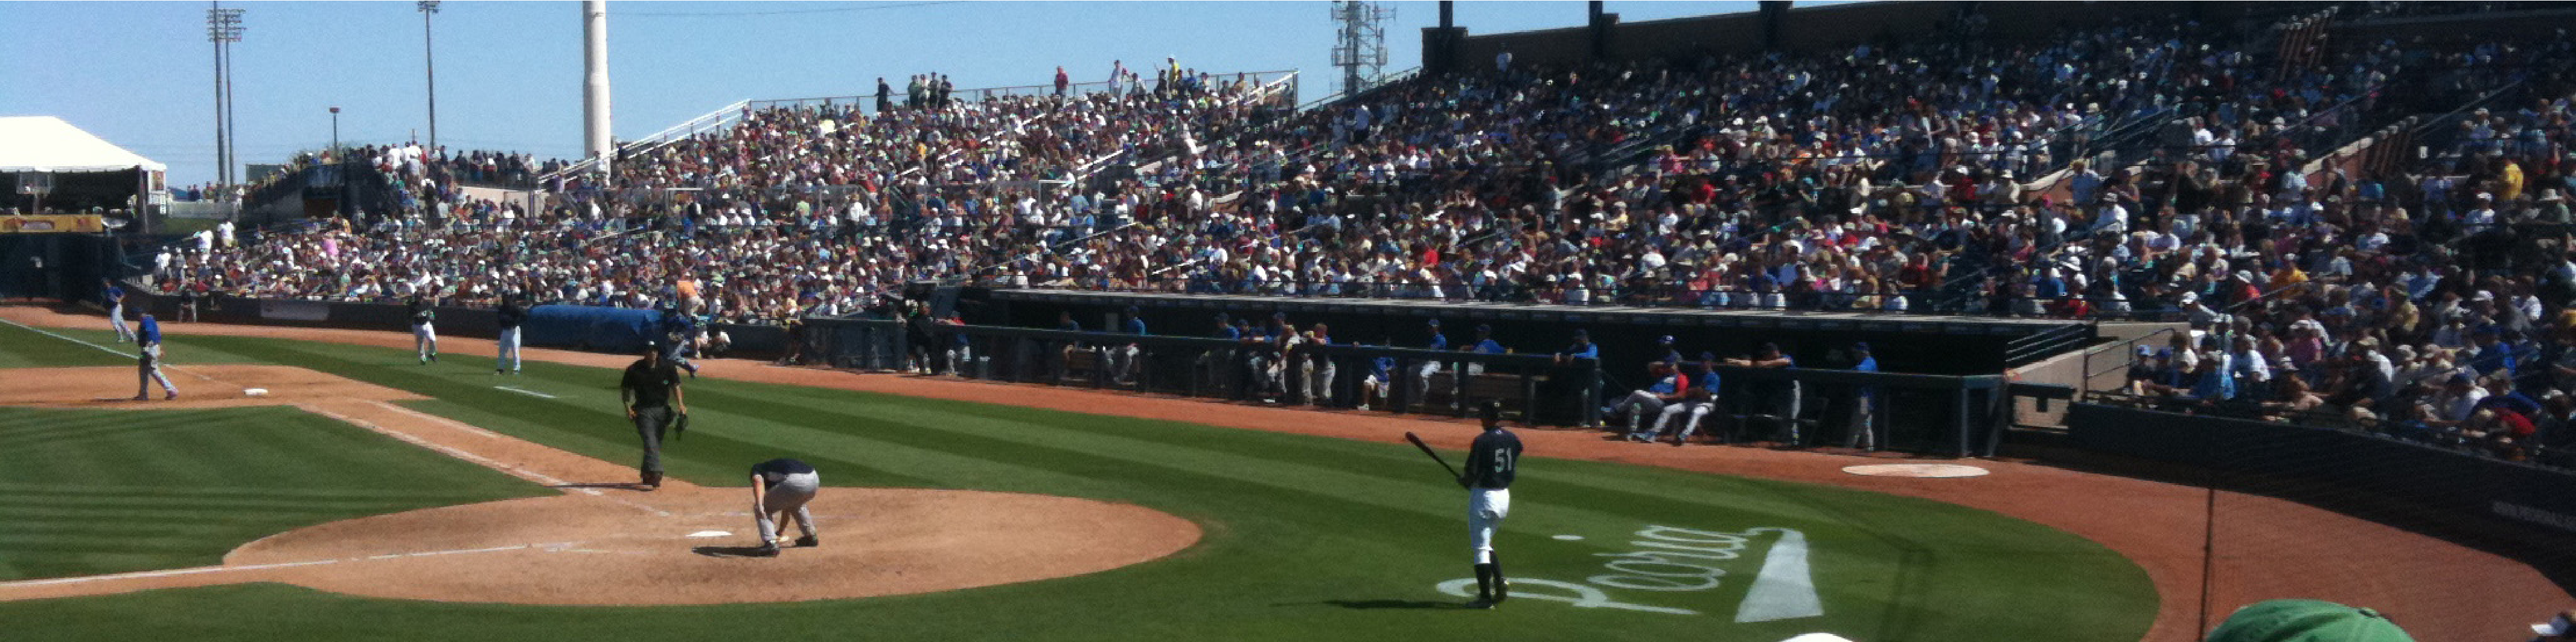
\includegraphics[height=1.5in]{images/sampleteaser}
%%   \caption{Spring Training 2009, Peoria, AZ.}
%% }

\maketitle


\begin{abstract}

Performance of interactive graphics walkthrough systems depend on the time
taken to fetch the required data from the secondary storage to the
main memory. It has been earlier established that a large fraction of this
fetch time is spent on seeking the data on the hard disk. In order to reduce
this seek time, redundant data storage has been proposed in the literature, but
the redundancy factors of those layouts are prohibitively high.  In this paper,
we develop a cost model for the seek time of a layout.  Based on this cost
model, we propose an algorithm that computes a redundant data layout with the
redundancy factor that is within the user specified bounds, while maximizing
the performance of the system.


\end{abstract}




%\begin{CRcatlist}
%  \CRcat{I.3.6}{Computer Graphics}{Methodology and Techniques}{Graphics data structures and data types};
%\end{CRcatlist}

\keywordlist

%% Use this only if you're preparing a technical paper to be published in the 
%% ACM 'Transactions on Graphics' journal.

\TOGlinkslist

%% Required for all content. 

\copyrightspace

\begin{figure}[t]
  \centering
  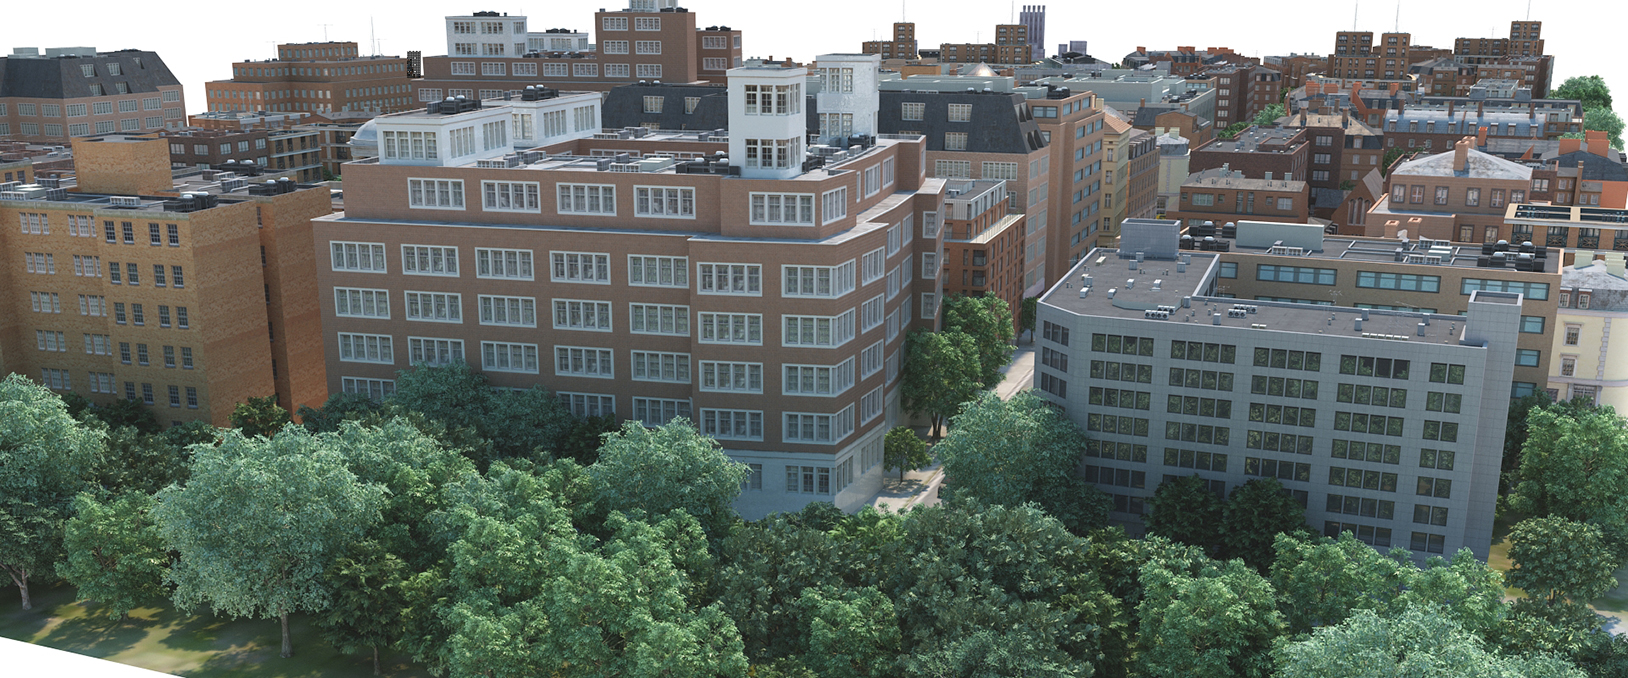
\includegraphics[width=\columnwidth]{densecity.jpg}
  \caption{Urban model: 100 million triangles, 12 GB. Using our method the walkthrough rendering performance for this model was significantly improved over existing methods. }
  \label{fig:model3}
\end{figure}

\section{Introduction}

%\subsection{Walkthrough Rendering}

In typical walkthrough systems, data sets consisting of hundreds of millions of
triangles and many gigabytes of associated data (e.g. walking through a virtual
city) are quite common. Rendering such massive amounts of data requires
out-of-core rendering algorithms that bring only the required data for
rendering into main memory from secondary storage. In this process, in addition
to the rendering speed, the data fetch speed also becomes critical for
achieving interactivity, especially when we handle large-scale data. In
general, data fetch speed depends on data seek time and data transfer time.
Transfer time depends only on the amount of data that is transferred. Seek time
is the time taken to locate the beginning of the required data in the storage
device and depends on different factors depending on the storage medium. \\
\\
For a hard disk drive (HDD), its seek time depends on the speed of rotating the
disk,
and the relative placement of the data units with respect to each other, also
called the data layout~\cite{Rizvi10}. For a solid state drive (SSD), this seek
time is usually a small constant and is independent of the location of the data
with respect to each other~\cite{SSD_perf08}. An earlier work utilized this
difference between SSD and HDD, and designed a data layout tailored for using
SSDs with the walkthrough application~\cite{ssdpaper}. There have been many
other techniques utilizing SSDs for various applications~\cite{FlashVM09}. SSD,
unfortunately, is not the perfect data storage and has its own technical
problems, including limited number of data overwrites allowed, high cost, and
limited capacity~\cite{Rizvi10}.  \\
\\
On the other hand, the HDD technology -- including disk technologies such as
CDs, DVDs, and Blu-ray discs -- has become quite reliable and inexpensive
thanks to their extensive verifications and testing, and is thus in widespread
use.  Even for massive data sets HDDs are still and will be
the preferred medium of storage for the foreseeable future~\cite{Rizvi10},
mainly
because of its stability and low cost per unit. As an example, according
to~\cite{pcmagarticle}, as of 2014, an HDD can cost \$0.08 per GB, while an SDD
can cost \$0.60 per GB. As a result, optimizing components of walkthrough
systems with HDDs is critical. In particular, addressing the seek time, the
main bottleneck of accessing data from HDDs, remains the main challenge for
interactive rendering of massive data sets. 
%In this paper, we leverage the
%inexpensive nature of HDDs to store redundant copies of data in order to reduce
%the seek time. 

%\subsection{Redundancy based data layouts}

In this paper, we leverage the inexpensive nature of HDDs to store redundant
copies of data in order to reduce the seek time. Adding redundancy in order to
improve the data access time is a classic approach, e.g.,
RAID~\cite{Patterson88}.  We are also not the first to consider redundancy for
walkthrough applications.  Redundancy based data layouts to reduce the seek
time were introduced in a recent work~\cite{singleseeklayout}, in which the
number of seeks for every access was reduced to at most one unit. However, in
order to achieve this nice property, the redundancy factor -- the ratio between
the size of the data after using redundancy to the original size of the data --
was
prohibitively high around 80. \\
\\
Another recent work \cite{optimizingredundancy} took the data transfer time, seek time,
and redundancy, and proposed a linear programming approach to optimize the data
transfer and seek time in order to satisfy the total data fetch time
constraint. In the process, redundancy was a hidden variable that was
minimized. Unfortunately, this approach does not directly model redundancy or
seek time, and thus can have unnecessary data blocks and unrealistic seek
times.
%\YOON{I think that we need to compare the current work against this work in a way in the .}. 

%\subsection{Main Contributions}
{\bf Main contributions:}
In this paper, we propose a model for seek time based on the actual
number of units
between the data blocks in the linear data layout. Using this model, and given
the spatial proximity of the data set for a walkthrough application, we develop
an algorithm to duplicate data blocks strategically to maximize the reduction
in the seek time, while keeping the redundancy factor within the user defined
bound. We will show that our greedy solution can generate both the extreme cases
of data layout with redundancy, namely the maximum redundancy case
(a layout where seek time is at most one) and the no-redundancy case (a simple
cache oblivious mesh layout with a potentially high seek time), as well as
reasonable solutions for redundancy factor constraints in between the extremes.
We show that the
implementation of our algorithm significantly reduces average delay between
frames and noticeably improves the consistency of performance and
interactivity.


\section{Related Work}
Massive model rendering is a well studied problem in computer graphics. Most of
the early works focused on increasing the rendering efficiency. At that time
the fundamental problem was not fitting the model into main memory, but
fully utilizing the speed of the graphics cards. Hence these works provided
solutions to reduce the number of primitives to be rendered while maintaining
the visual fidelity. These solutions included level-of-detail for geometric
models \cite{Luebke02}, progressive level of detail
\cite{Hoppe:98b,Hoppe:97,Hoppe:96,SG:01}, and image based simplification
\cite{ACWBZEHHSBWBM:99}. Soon thereafter the size of main memory became the
bottleneck in handling ever increasing sizes of the model. Hence memory-less
simplification techniques \cite{LT:99}  and other out-of-core rendering systems
\cite{Silva02,VM:02} emerged in which just the limited amount of required data
that needs to be processed and rendered was brought from the secondary storage
to main memory. \\
\\
The speed at which this data
could be brought from the secondary to main memory in these out-of-core
algorithms is limited by the data bus speed, disk seek time, and data transfer
time. These limitations could be ameliorated to some extent by
better cache utilization that would increase the utilization of data that is
brought to main memory and thus reduce the number of times the disk read is
initiated. This meant that subsequent works focused on cache aware
\cite{ssdpaper} and cache oblivious data layouts
\cite{cacheobliviouslayout,YOON:2006:MeshLayout} on the disk to reduce the
data fetch bottleneck. Our work falls under this class of algorithms that
reduces the data fetch time. \\
\\
Redundancy based data layouts were mentioned in
\cite{Patterson88,singleseeklayout,optimizingredundancy} as potential solutions
to this problem of reducing seek time. In particular
\cite{optimizingredundancy} presented an algorithm that limits the amount of
redundancy required, but there were major drawbacks. First, it provides a
grouping of data units for each seek, but it does not provide a data layout.
This is because it does not relate one data group with another.
Such an approach could easily result in unnecessary data
block duplications since groups of data units can overlap with each other. There is no mechanism in the integer programming solver to detect whether this redundancy is necessary because of some scene context or simply created blindly due to local optimization. The redundancy minimization is thus not modeled after
physical representation of the data layout on the disk. The second major
drawback is that the model for seek time is also not based on physical reality.
Typically, seek time depends on the relative distance on the disk between the
last data unit accessed and the data unit currently being requested. However,
in \cite{optimizingredundancy}, seek time is simplistically modeled,
% as counting
%the number of seeks, 
independent of the number of data units between them. For example,
%means that 
irrespective of whether the requested data blocks are adjacent to
each other or far apart, this model would assign the same cost for both
layouts. Our approach
aims to address these issues. 


\begin{figure}[t]
  \centering
  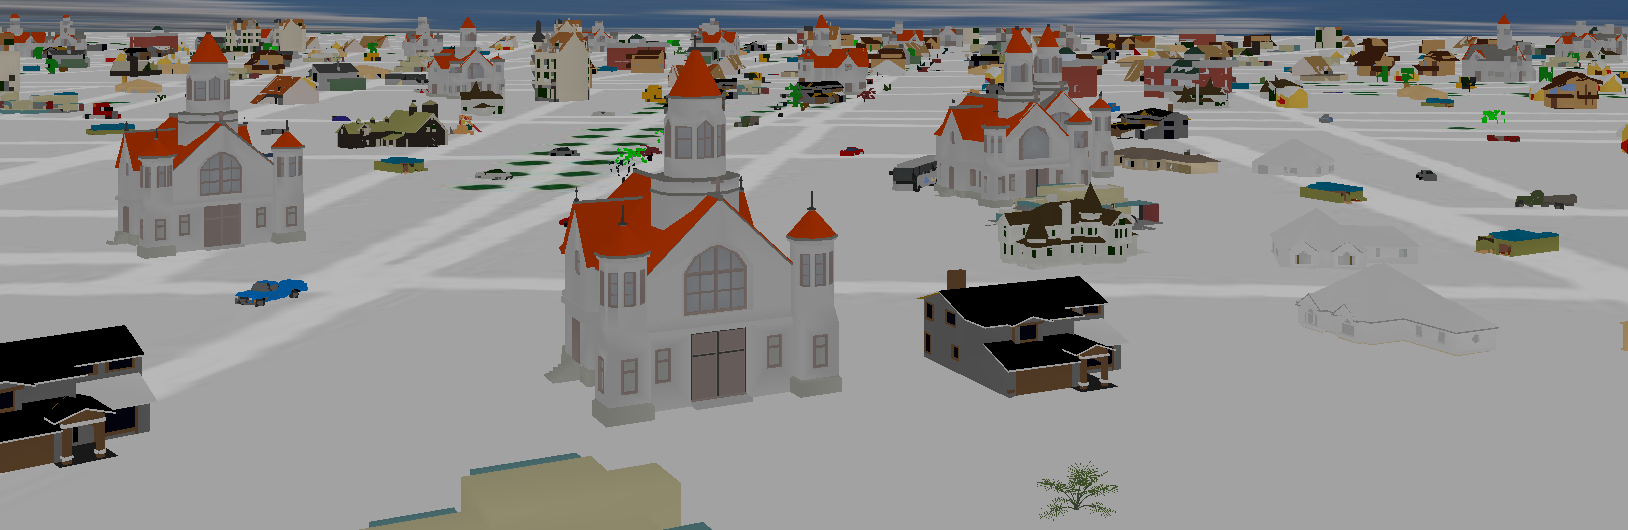
\includegraphics[width=\columnwidth]{city.png}
  \caption{City model: 110 million triangles, 6 GB }
  \label{fig:model1}
\end{figure}




\section{Redundancy-based Cache Oblivious Data Layout Algorithm}

\subsection{Definitions}

Let us assume that the walkthrough scene data, including all the levels of details of the model, are partitioned into equal sized data blocks (say 4KB) called data units. This is the atomic unit of data that is accessed and fetched from the disk. Typically, vertices and triangles that are spatially together (and belong to the same level of detail), have high chances of being rendered together, and hence can be grouped together in a data unit. All the data units required to render a scene from a viewpoint is labeled as an {\em access requirement}. In order to minimize the number of access requirements, the navigation space in the walkthrough scene, which defines the space of all possible view points, is partitioned into grids and all the viewpoints within each grid is grouped together to define one access requirement. Thus the number of grid partitions define the number of access requirements. Clearly, primitives in a data unit can be visible from many viewpoints, and hence that data unit will be part of many access requirements. \\
\\
That was one example of data units and their access requirements. In general, the access requirements are determined by the application and are meant to be sets of data units that are likely to be accessed together. Given a linear ordering of data units that may eventually be the order in which they are stored in the hard drive, for an access requirement $A$, the total span of $A$ is the total number of data units between the first and last data units that use $A$. If a data unit is not required by $A$ but lies between the first and last unit of $A$ then it is still counted in the span of $A$. Figure \ref{singleAR} shows a set of data units and explicitly labels the blue access requirement in this set. The total number of data units between the first and last blue unit is 14 thus that is the total length of the blue access requirement.\\
\\
\begin{figure}[ht]
\centering
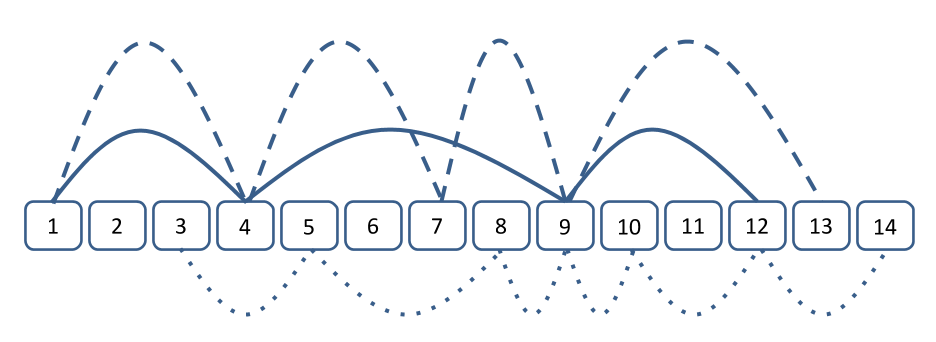
\includegraphics[width=3in]{Figure1-AccessReqs.png}
\caption{Illustration of linear order of data units and three example access requirements.
The lines connect data blocks that belong to the same access requirement
and represent parts of the span of an access requirement.}
\label{singleAR}
\end{figure}

\subsection{Seek Time Measure}
Given a linear order of data units and the access requirements, and assuming that each access requirement
is equally likely to be used, we would like to estimate the seek time for that application.
For each access requirement the read head of the hard disk has to move from the first data block to the last
irrespective of whether the intermediate blocks are read or skipped. Hence the span of an access requirement
is a measure of seek time - time taken to seek the last data unit starting from the first data unit.
Let $I$ be the set of access requirements and $A_i$ represent the span of the access requirement $i$.
Then estimated total seek time EST is given by 
\[
EST = \sum_{i \in I}{A_i}
\]
It is interesting to note that \cite{cacheobliviouslayout}
used span to measure the expected number of cache misses.
Typically, with every cache miss, the missing data will be sought in the disk and fetched,
thus adding to the seek time. Hence using span to measure the seek time is justified.


\subsection{Algorithm Overview}

In \cite{cacheobliviouslayout}, the only allowed operation on the data units is
the move operation and the optimal solution is computed using only that
operation. For our purposes, we are allowed to copy data units, move them, and
delete them if they are not used. Using these operations, our goal is to minimize EST
while keeping the number of redundant copies as low as possible. After constructing a cache oblivious layout 
of the data set to get an initial ordering of data units, we copy one data unit to another location, and reassign 
one or more of the access requirements that uses the old copy of the data unit to the new copy, such that the EST is reduced. 
If all the access requirements that used the old copy, now use the new copy of the data unit, then the old copy is deleted. 
We repeat this copying and possible deletion of individual data units until our redundancy limit has been reached. \\
\\
{\bf Blocks to Copy:} Note that the span of an access requirement does not
change by moving an interior data unit to another interior location. Cost can
be reduced only by moving the blocks, i.e. data units, that are at the either ends of the access
requirement. This observation greatly reduces the search space of data units to
consider for copying. For the sake of simplicity of the algorithm, we operate
on only one data block at a time. \\
\\
{\bf Location to Copy:} Based on the above observation, given an access requirement, we can possibly move the beginning or the end data units of an access requirement to its interior. This will reduce its span, thus reducing the EST for the layout. However, if the new location of the data unit is in the span of other access requirements, it increases the span of those accesses by one unit. We thus want to find a location in the span of the access requirement under consideration but is in the span of the least number of other access requirements. Such a location is identified using a simple linear search through the span of the access requirement. \\
\\
{\bf Moving versus Copying:} A data unit can be accessed by multiple access
requirements. If that data unit is an extremal unit for an access
requirements, and if it is moved to its interior, it affects span of those access
requirements that use the
same data unit. That is the main reason that we are copying and not moving
these data units. 
By copying the data unit the other access requirements can
still access it in its old location. The only increase in span for those access requirements would possibly be an extra unit resulting from the copying itself but it would not come from having to use the new copy.
Nevertheless, if by using the new copy the span of one or more of the other
access requirements reduces, then those access requirements should use the new
copy instead of the old copy. If all the access requirements use the new copy
so that the old data block is not used by any access, then it can be deleted. In
this later case, we are really moving the data block. \\
\\
{\bf Data Block processing order:} 
We now need to figure out how to use this
information to decide in what order the copying should be done. When considering the order we are only considering cases where we are copying and not the cases where we are moving. This is because copying adds a space cost so we need a way to decide in what order it should be done whereas moving does not have that cost. For each data
unit, its total benefit is the amount that is reduces the total seek time
($EST$). For a given data unit to be copied to a specified location, let $k_i$
be the benefit to access requirement $i$ that is attached to the data unit. We
will say that $k_i=0$ if the access requirement will use the old copy and not have its span increased by the addition of a new copy, $k_i=-1$ if the access requirement will use the old copy but still have its span increased, and
$k_i>0$ if the access requirement will use the new copy. Let $I$ be the set of
access requirements that use the data unit. Let $J$ be the set of access
requirements not in $I$ whose span overlaps our data units. We can now describe
the benefit, the reduction in seek time, as follows:
\[
Benefit = -\Delta EST = \sum_{i \in I} k_i - |J|.
\]
Before doing any actual copying, we compute the above described benefit for
each start and end data unit for each access requirement. We store all the
benefits into a binary search tree, i.e. a heap, sorted in descending order by benefit
amount. That way we will easily be able to choose the data unit that provides
the most benefit in expected seek time. We will also make a special list $L$ of
cases where a data unit is copied and then can be deleted, because by doing
that, all the access
requirements will benefit. \\
\\
Because doing the moving for the list $L$ does not increase the storage, we will first go through that list and perform those moves. After each of the moves we have to recompute the costs and update the tree and list. Once $L$ is empty we will take the data unit in the binary search tree that provides the most benefit and perform the copy. We will then recompute $L$ and the binary search tree. We will continue to do those steps until we have run out of available space for redundancy. As a summary, the psuedo-code of this algorithm is shown as algorithm \ref{pseudocode}.

\begin{algorithm}
\YOON{The current pseudo code seems to be very long and verbose. This can give an impression that the algorithm is complex, while the proposed one is very simple.}
Start with the data units which each with at least one access requirement (AR)\;
Initialize AR, heap H, and list L\;
\For{each data unit}{
	Find number of overlapping access requirements and store the number with the data unit\;
}
\For{each AR P's head and tail data units U}{
	make old copy list L' empty\;
	\eIf{U is head data unit}{
		Let S = data unit in P after U\;
	}{
		Let S = data unit in P before U\;
	}
	Set BENEFIT=distance(S,U)\;
	Let U' be the potential copy of U\;
	Search data units between S and U for min number of overlapping ARs and put U' there\;
	make old copy list L', the list that stores the ARs that will use the old data unit, empty\;
	\For{each AR T that also uses U}{
		\eIf{T will be shorter by using U'}{
			Add T's benefit to BENEFIT\;
		}{
			Add T to list L'\;
		}
	}
	Add BENEFIT to heap H\;
	\If{L' is empty}{
		add U to list L\;
	}
}
\While{BREAK has not been called}{
		\While{L is not empty}{
			Take out random element and move the data unit\;
			Update heap H and list L\;
		}
		\eIf{there is more space for redundancy}{
		pop best element U from H\;
		copy U to its destination\;
		update nodes in H and entries in L for affected access requirements\;
		update H and L\;
		}{ call BREAK}
}
\caption{Pseudo-code for our algorithm}
\label{pseudocode}
\end{algorithm}


\section{Complexity Analysis}

We now analyze the running time and storage requirements of our algorithm. Let
$N$ be the number of data units and $A$ be the number of access requirements.
We will use $k$ as the average span of a single access requirement. Let $r$ be the redundancy factor limit specified by the user so that $O(rN)$ units can be copied. For the sake of analysis each data unit will have $O(A)$ access requirements attached to it and $O(A)$ access requirement spans that overlap it even though the actual number will likely be lower in both cases. 

{\bf Time Complexity:} The construction of the heaps $E_M$ and $E_C$ involves
computing the benefit information for all $A$ access requirements and inserting
each one into the heap. For a single access requirement, computing the benefit information of moving or copying one of its data units involves scanning each data unit in its span. We justify
this approach which takes $O(k)$ operations in Appendix A. Calculating $\sum_{s\in S}\Delta{A_s}$ and $\sum_{t\in T}\Delta{A_t}$ will take $O(A)$ operations since there are $O(A)$ access requirements to potentially have to sum over. Inserting this
benefit information into the heap takes $O(log (A))$ operations. In total then it takes $O(k + A + logA)$ or $O(k + A)$ operations per access requirement to get the benefit information. The initial construction thus takes $O(A(k+A))$ operations. \\
\\
After the initial construction, the move and copy loops are executed. In every iteration of move or copy, an element from the top of the heap is removed and processed, the benefit function is recalculated for affected access requirements, and the heap is updated. There are potentially $O(A)$ overlapping access requirements whose benefit information needs to be recalculated. As shown above, for each of these access requirements $O(k+A)$ operations are required to perform the recalculation and update the heap. Each iteration of move or copy thus takes a total of $O(A(k+A))$ operations.\\
\\
For simplicity we will assume that the move loop runs $O(N)$ times total. This comes from the fact that the
cache oblivious layout \cite{cacheobliviouslayout} should be a good
approximation so the number of moves that would be useful should be
limited. There are $O(rN)$ copies made so there are that many iterations of the copy loop. We thus
can assert that there are $O(rN + N)$ iterations of the move or copy loops. We can simplify this to $O(rN)$ operations since $r \geq 1$. In total then the moving and copying loops will take
$O(rNA (k + A))$ operations, which is also the running time for the whole algorithm. \\
\\
{\bf Space Complexity:} During the run of the algorithm, we have to store the number of overlapping spans at each data unit, which will require $O(N)$ storage. We will also have to store a heap of access requirements, which can be stored using $O(A)$ space. We also have a list of access requirements and that information will take up $O(A)$ space. In total we thus have $O(A + N)$ storage space used during the run of the algorithm. 


\section{Experimental Results}

\begin{figure}[ht]
  \centering
  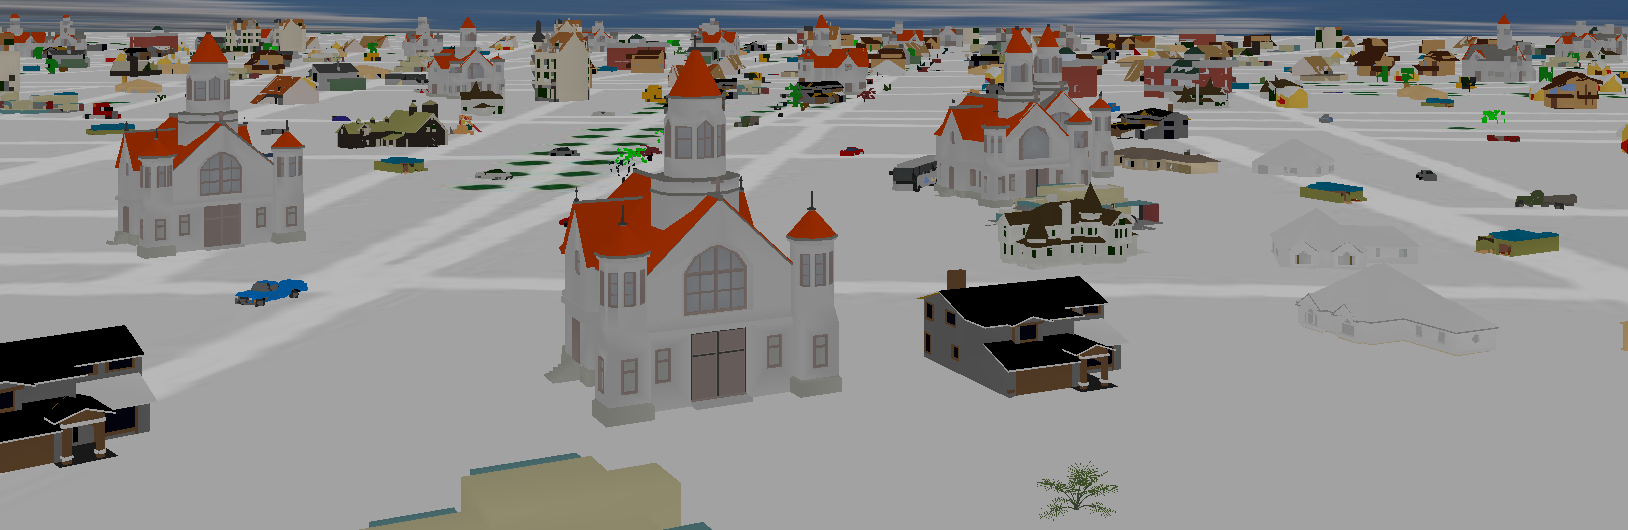
\includegraphics[width=\columnwidth]{city.png}
  \caption{City model: 110 million triangles, 6 GB }
  \label{fig:model1}
\end{figure}

\begin{figure}[ht]
  \centering
  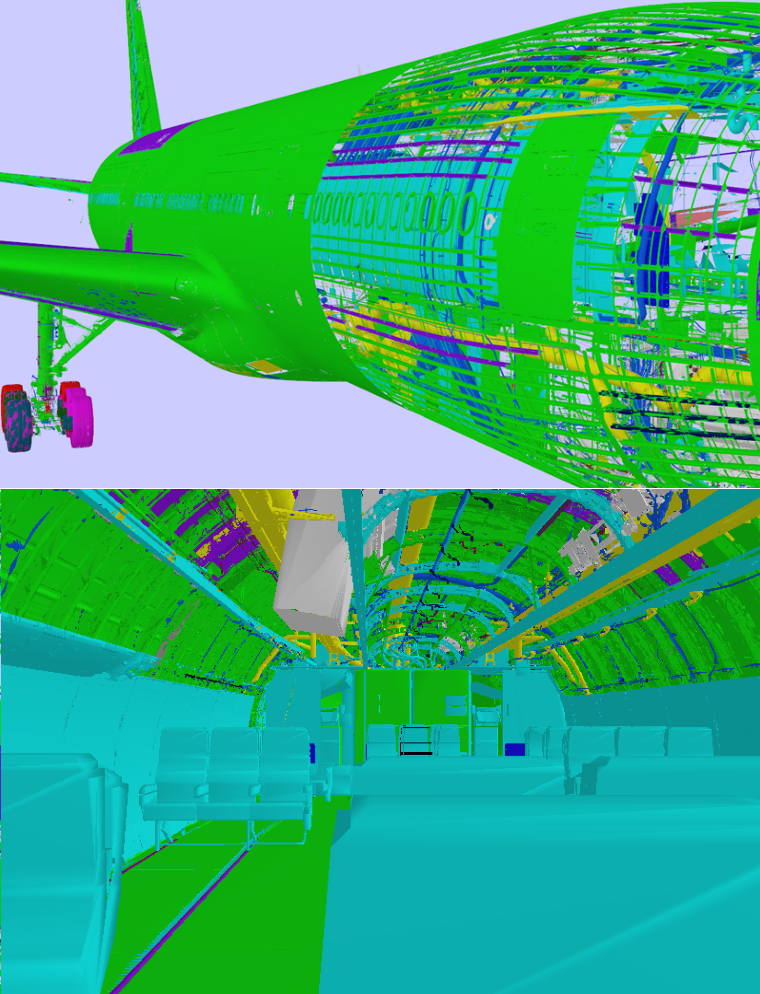
\includegraphics[width=\columnwidth]{BoeingModel.pdf}
  \caption{Boeing model: 350 million triangles, 20 GB. Overview of model (top) and model detail (bottom)}
  \label{fig:model2}
\end{figure}

\begin{figure}[ht]
  \centering
  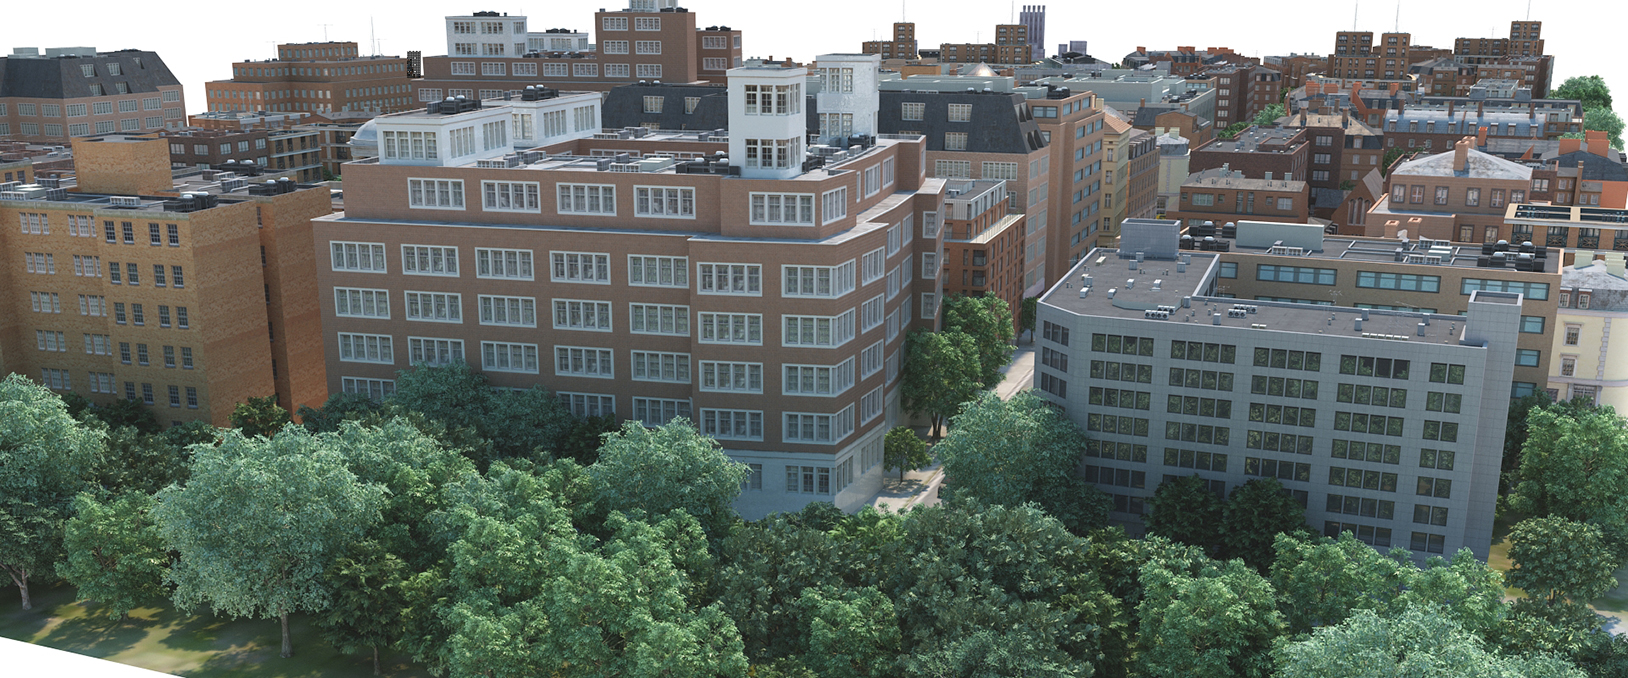
\includegraphics[width=\columnwidth]{densecity.jpg}
  \caption{Urban model: 100 million triangles, 12 GB }
  \label{fig:model3}
\end{figure}


\textbf{Experiment context:}
In order to implement our algorithm, we used a workstation that is a Dell T5400 PC with Intel (R) Core (TM) 2 Quad and $8GB$ main memory. The hard drive is a 1TB Seagate Barracuda with 7200 RPM and the graphics card is an nVIDIA Geforce GTX 260 with 896 MB GPU memory. The data rate of the hard drive is $120$ MB/s and the seek time is a minimum of $2$ ms per disk seek.\\
\\
\textbf{Benchmarks:}
We use three models to perform our experiments, each model represents a use
case or scenario. The City model (Figure \ref{fig:model1}) is a regular model
that can be used in a navigation simulation application or virtual reality
walkthough. The Boeing model (Figure \ref{fig:model2}), on the other hand,
represents scientific or engineering visualization applications. The Urban
model (Figure \ref{fig:model3}) has texture attached to it, which is commonly
used in games. By comparing performance of cache-oblivious layout without
redundancy~\cite{cacheobliviouslayout} to our method using redundancy on these three models, our goal
is to show that the redundancy based approach can achieve more stable and generally
better performance on different real time applications. \\
\\ To apply our method on these large-scale models, we had to find a proper set
of access requirements. In general, that question is deep enough that it can be
discussed as a separate research topic. Here, however, we had good performance
using only simple schemes for creating access requirements. Each model ended up
having a separate scheme. Nonetheless, an access requirement represents a set
of data that is highly likely to be accessed together. \\
\\
For the City model, a 2D grid is used to divide the space into square cells. For each pair of adjacent cells, the difference of the data is considered as an access requirement\YOON{Difference is access requirement? Odd. I guess that you are using pairs as accesses, and the diff. means their length in the 1 D layout?}. By propagating this rule, access requirements are created, and the number of them is determined by the resolution of the grid. \YOON{How many access requirement do you have in the end? For each cell, do you create an access requirement? Also, explain why you adopt this way of creating access requirement.} \\
\\
For the Boeing model, the predefined objects are used as a conceptual level to create access requirements. Samples of view positions are distributed across the model. For each sample, four fixed directions and four random directions are considered. Objects visible from this position in any one of these eight directions are added to access requirement for this specific sample. The density of these samples depends on the complexity of local occulders to reduce load of each access requirement, i.e. more samples are distributed to places with more complex geometry. \\
\\
The Urban model is different from the previous two in a way that it involves textures. Building heavy redundancy of textures increases the total size of the dataset significantly, while keeping textures away from redundancy leads to inevitable long seek time, which is completely against the philosophy of this work. To solve this problem, we applied a spatial Lloyd’s clustering \cite{lloydclustering} on objects. By moving centers of clusters, we look for a solution such that each cluster involves almost same amount of texture data. Between clusters, textures can be redundantly stored, but within each cluster, texture data are stored uniquely. In this way, each cluster is used as an access requirement.  \\
\YOON{Mention how long does it take to compute the redundancy layout for each model.}
\\
\textbf{Results:}
Figure \ref{fig:resultall} shows the results of delays caused by fetching data on the experimental models we used. We compare the results of a cache-oblivious layout without redundancy and one with redundancy. For the layout with redundancy, we set the redundancy factor equal to 4.2. This factor was chosen because as can be seen in Figure \ref{fig:statistic}, it had considerably better performance than lower redundancy factors and did not have significantly worse performance than higher redundancy factors. A factor of 4.2 is also still practical, as the largest model we tested, the Boeing model, becomes 84 GB which is still acceptable given the large capacity of modern secondary storage devices.\\
\\
It is clear that the performance of the layout with redundancy has generally shorter delays than the cache-oblivious layout without redundancy. As can be observed from the results, although the layout with redundancy does not eliminate delays for most of sample points on the walkthrough path, it reduces delays to a small range and keeps the performance more consistent. This is the benefit we get from using our algorithm which adds redundancy. Since the algorithm tends to eliminate seeks with longer seek time first, in practice the larger delays are avoided.
\begin{figure}[ht]
\centering
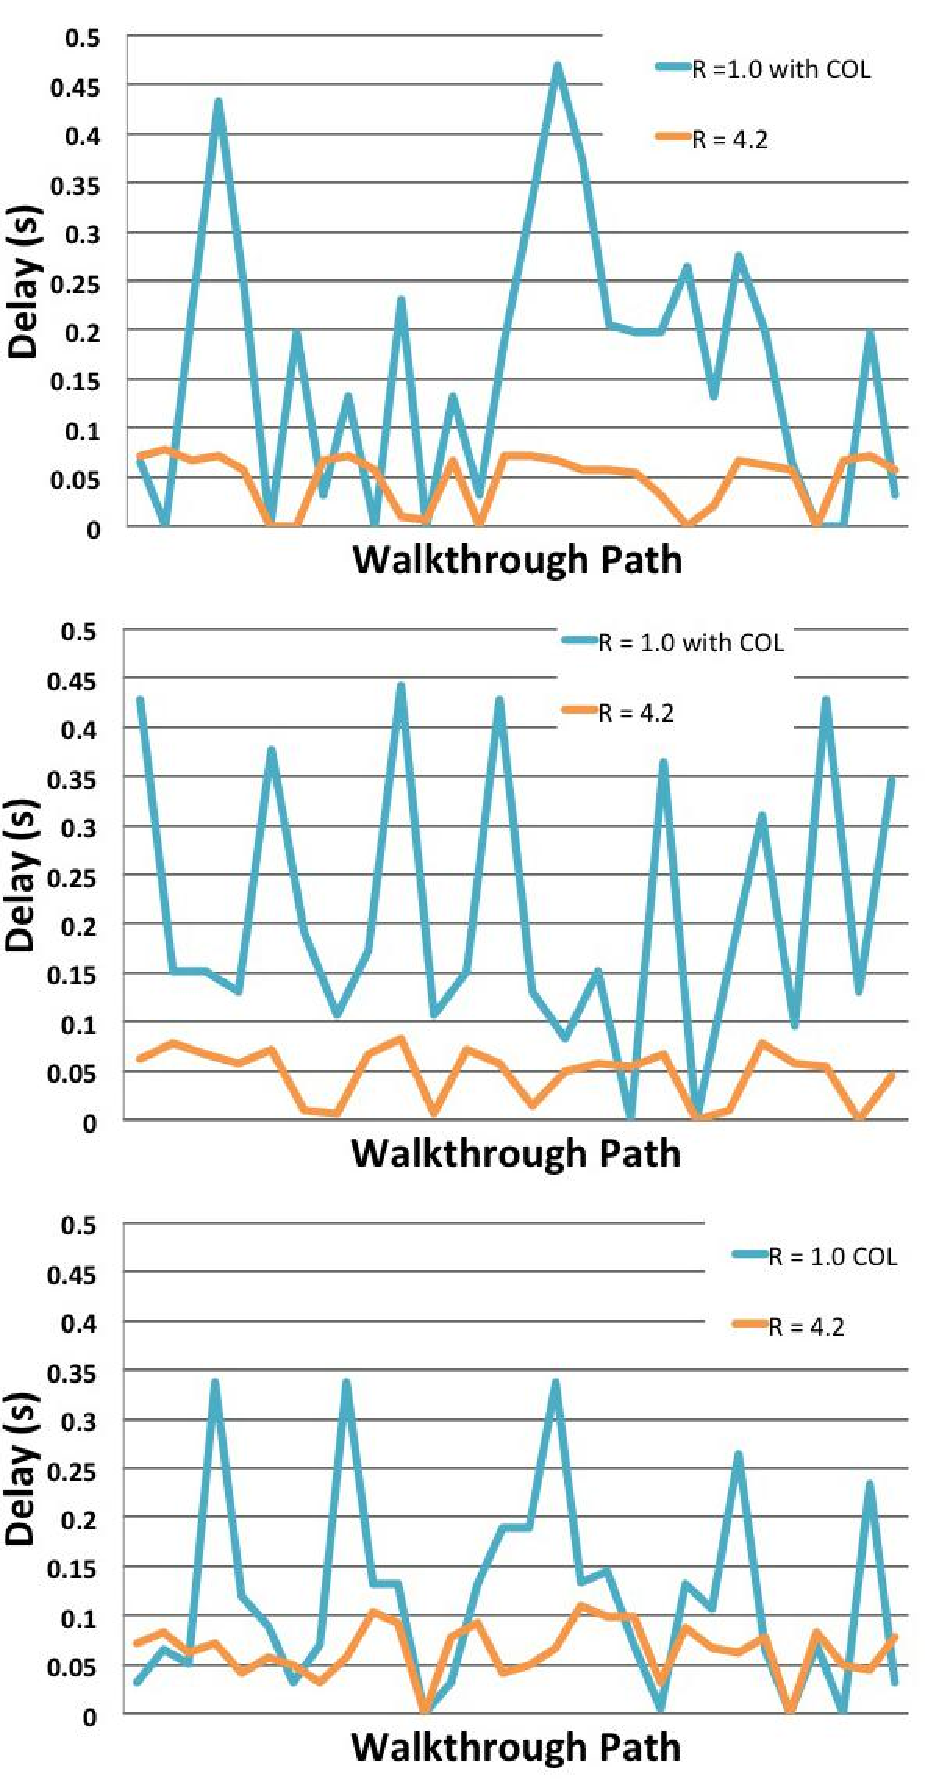
\includegraphics[width=\columnwidth]
{comparison_to_COL_all.pdf}
  \caption{Statistics of delays caused by the fetching processes for the City model (top), the Boeing model (center), and
the Urban model (bottom), with and without redundancy. }
  \label{fig:resultall}
\end{figure} 

\begin{figure}[ht]
\centering
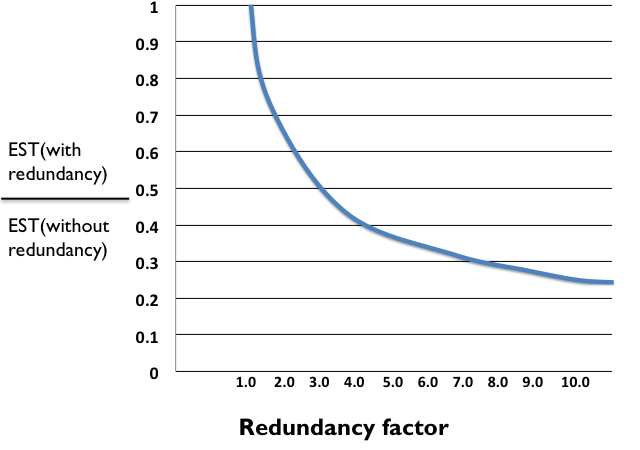
\includegraphics[width=\columnwidth]{statistic.png}
  \caption{Plot of the ratio of the EST of layout with redundancy over the EST of cache-oblivious mesh layout without redundancy. }
  \label{fig:statistic}
\end{figure} 

\begin{figure}[ht]
\centering
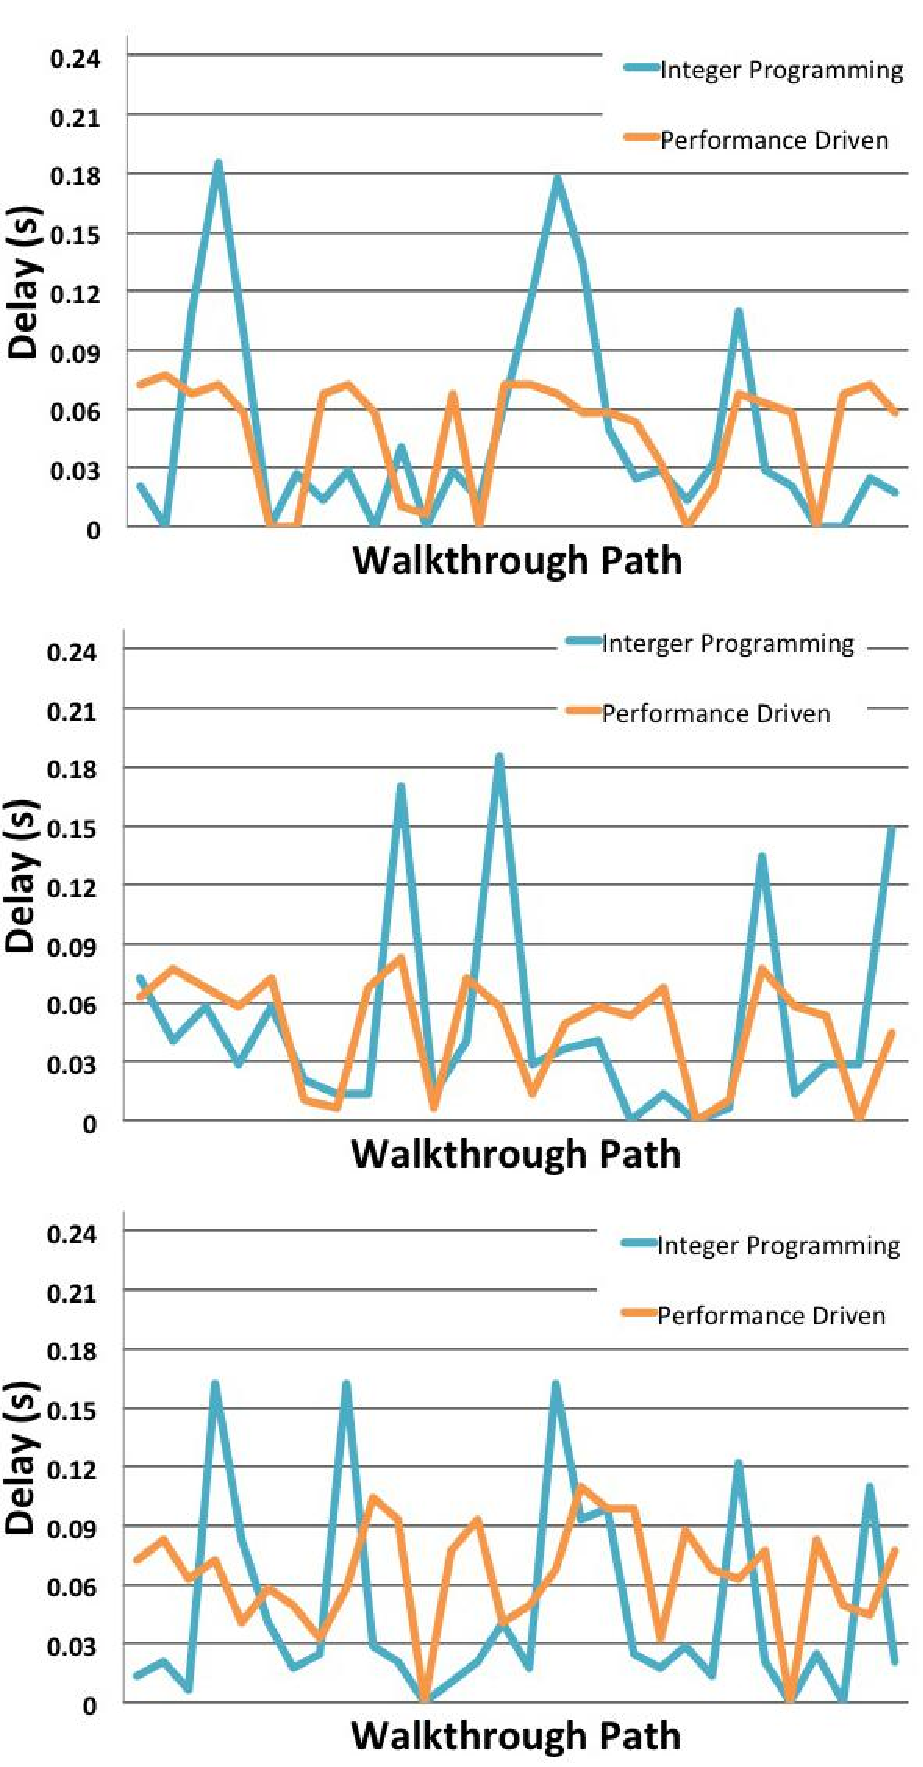
\includegraphics[width=\columnwidth]
{comparison_to_lin_programming_all.pdf}
  \caption{Statistics of delays caused by the fetching processes for the City model (top), the Boeing model (center), and
the Urban model (bottom), using integer programming and our method}
  \label{fig:linProgramComparison}
\end{figure}

When we compare our method to the one in \cite{optimizingredundancy}, there is a performance benefit that can be observed in Figure \ref{fig:linProgramComparison}. Additionally in \cite{optimizingredundancy}, the user does not have any control over the final redundancy factor however each time we duplicate one data unit, we can halt it if the redundancy factor reaches a certain threshold. This helps us create data layouts with arbitrary redundancy factors. We use this fact to test different redundancy factors and see their results. In Figure \ref{fig:statistic}, we show the results of using layouts with redundancy factors that range from 1.0 to 10.0. The y-axis in this figure is the ratio of the estimated seek time (EST) of the layout with redundancy over the EST of the layout without redundancy. This value starts at 1.0 where redundancy factor is 1.0, meaning no redundancy, and decreases as redundancy factor goes larger. We can see that the rate of this decrement is not constant, and the benefits we gain at beginning are larger than the ones we get later. This implies that most of the performance improvement resides at the earlier phase of raising redundancy factor. This implies that it is worthwhile to limit the redundancy factor used because after a certain point you are using much more secondary storage space without improving seek time by much. It also implies that our algorithm dramatically reduces seek time in practice by using only small redundancy factors. 




\section{Cache Oblivious Layout With and Without Redundancy}

In the algorithm, we make a heap of data units that will reduce seek time by
just moving instead of copying them. We perform these moves first before
working with data units that need copying. This initial step will produce a
better solution than proposed by \cite{cacheobliviouslayout} without adding
redundant units. This result is possible mainly because our optimization
algorithm searches wider sets of potential locations for moving cases in an
efficient manner.
%mowhere data
%units are close to each other but in hierarchically different blocks in
%\cite{cacheobliviouslayout}. 
To show this, consider a case where we have two
access requirements of 5 data units each. Figure \ref{YoonImprovement} shows an
example of that kind of layout. In the middle of that figure is the result of
using the cache oblivious layout. Because it hierarchically constructs blocks
and arranges the units in each block, it does
not detect that the
units with the black access requirement can be grouped together. On the other
hand, the algorithm we propose would shorten the black access requirements
without adding redundancy, as shown in the bottom of that figure.

\begin{figure}[ht]
\centering
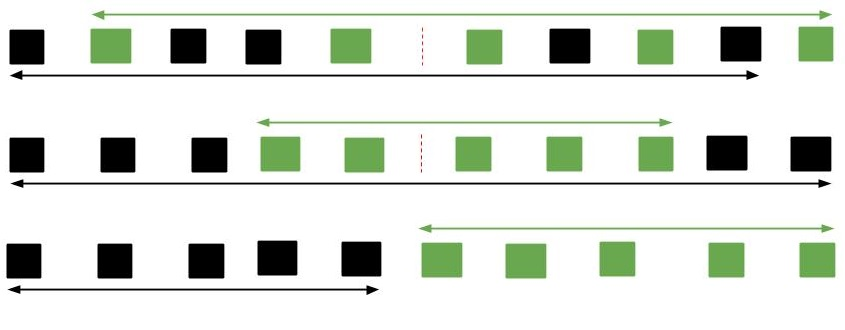
\includegraphics[width=\columnwidth]{ImprovementOverYoon.jpg}
\caption{Example of two access requirements of 5 data units each. The red line represents the boundary between blocks in the cache oblivious layout hierarchy. The original layout (top), cache-oblvious layout (middle), as well as the layout after running our algorithm (bottom) is shown.}
\label{YoonImprovement}
\end{figure}

The algorithm in \cite{cacheobliviouslayout} did not necessarily produce the best cache oblivious layout. However, even if we had the best layout without redundancy, we would actually achieve a better seek time using redundancy. We have such an example with Figure \ref{fig:startingProb}. As can be seen in the figure, the total seek time is 7 units which turns out to be the minimum possible seek time without redundancy, as found through a brute-force search. With redundancy, the total seek time is the minimum required which is 6 units. While a reduction from 7 to 6 units may not seem dramatic, when this result is scaled up to the hundreds of millions, this makes a big difference in seek time, which we saw in practice.\\

\begin{figure}[h!]
\centering
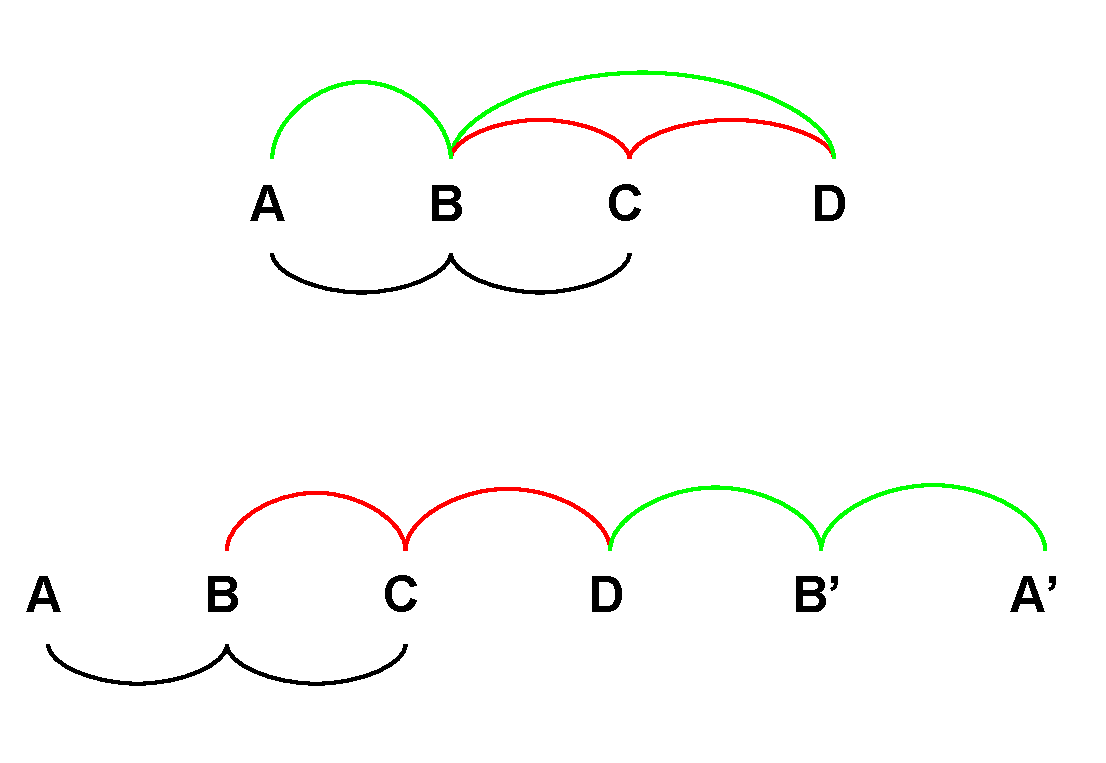
\includegraphics[width=\columnwidth]{DataLayoutPaper_TheoryLayouts.pdf}
\caption{Data Units with varying access requirements on the top. The letters represent data units and each color represents a different access requirement. It is laid out in its optimal layout without redundancy on top. Its optimal layout with redundancy is shown at the bottom.}
\label{fig:startingProb}
\end{figure}



\section{Conclusion and Future Work}

Given the data units, access requirements, and the desired upper bound on
redundancy factor, we have proposed an algorithm that would create a cache
oblivious layout with the primary goal of reducing the seek time through
duplicating the data units. We proposed a cost model for estimating the seek
time, and in our algorithm we can move or copy data units in appropriate
locations such that it reduces the estimated seek time.  We have shown that
such a layout significantly improves both the performance and consistency of
interactivity in massive model walkthrough applications.  \\ \\
Our proposed redundant storage of data may limit editing and modification of data because the data has to be modified at all copies. However, we foresee no problem in recomputing and updating the layout due to this modification using our algorithm since every iteration in our algorithm just assumes a layout and improves on it. After data modification, we can delete/modify the relevant data units, update the access pattern and run a few iterations of our algorithm to get a better layout. In other words, our algorithm is incremental and can be used for dynamic data sets also which might be a result of scene editing and modification.\\
\\
{\bf Limitations and future work:}
Our cost model does not take account distance between access requirements. We only take into account distance between data units in the same access requirement and we do not consider the seek time between access requirements. If we do take this account in our model, then if we are given information as to which access requirement is more likely to be used before or after another access requirement we would have an even more accurate model for seek time.



\bibliographystyle{acmsiggraph}
\bibliography{finalPaperRefs}

\end{document}
